%%%%%%%%%%%%%%%%%%%%%%%%%%%%%%%%%%%%%%%%%%%%%%%%%%%%%%
\section{The Standard Model}\label{secSM:ch1}

The Standard Model, SM, of particle physics constitues humanity's latest attempt at describing our universe in a calculable way. The basic premise being, the entire universe is compised solely of; 6 types of quark and 6 types of lepton, which comprise matter, and the guage bosons, which mediate the 3 (this theory does not yet encompass gravitaion) fundamental forces; The strong and weak nuclear interactions and electromagnetism. 


Various attempts have been made to unify the fundamental forces under one theory, thusfar the electromagnetic and weak interactions have been united by electro-weak theory. 

The Standard electroweak model can be described $SU(2) x U(1)$ mathematically.

The  $SU(2) x U(1)$ guage group is a convolution ( $<- $That is not the right word...) of the special unitary symmetry group $SU(2)$ describing 3 mixed vector bosons, $W_{-}$ $W_{+}$ $Z_0$, carriers of the weak nuclear force and the unitary gauge group $U(1)$ , describing the lonely photon, of the electromagnetic interaction.

The standard model of the strong interaction is known as quatum chromodynamics, QCD, described by the special unitary group $(SU(3)_f)$, where the flavours of quark are the physical manifestation of the symmetry group.

The SM also contains a Higgs boson, an excitation of a scalar Higg's field, which gives rise to spantaneous symmetry breaking of the electroweak theory, providing the particles with mass, but I won't get into that. 

The quarks and leptons are arranged in generations according to their relative masses, as shown in Figure \ref{fig:SM}. Nuclei in ordinary matter are composed solely of $1^{st}$ generation particles, up and down quarks, bound by gluons. Neutral atoms contain an equal number of protons (composed of 2 up quarks and a down quark) and electrons, $1^{st}$ generation leptons. There 



\begin{figure}[htb]
\centering
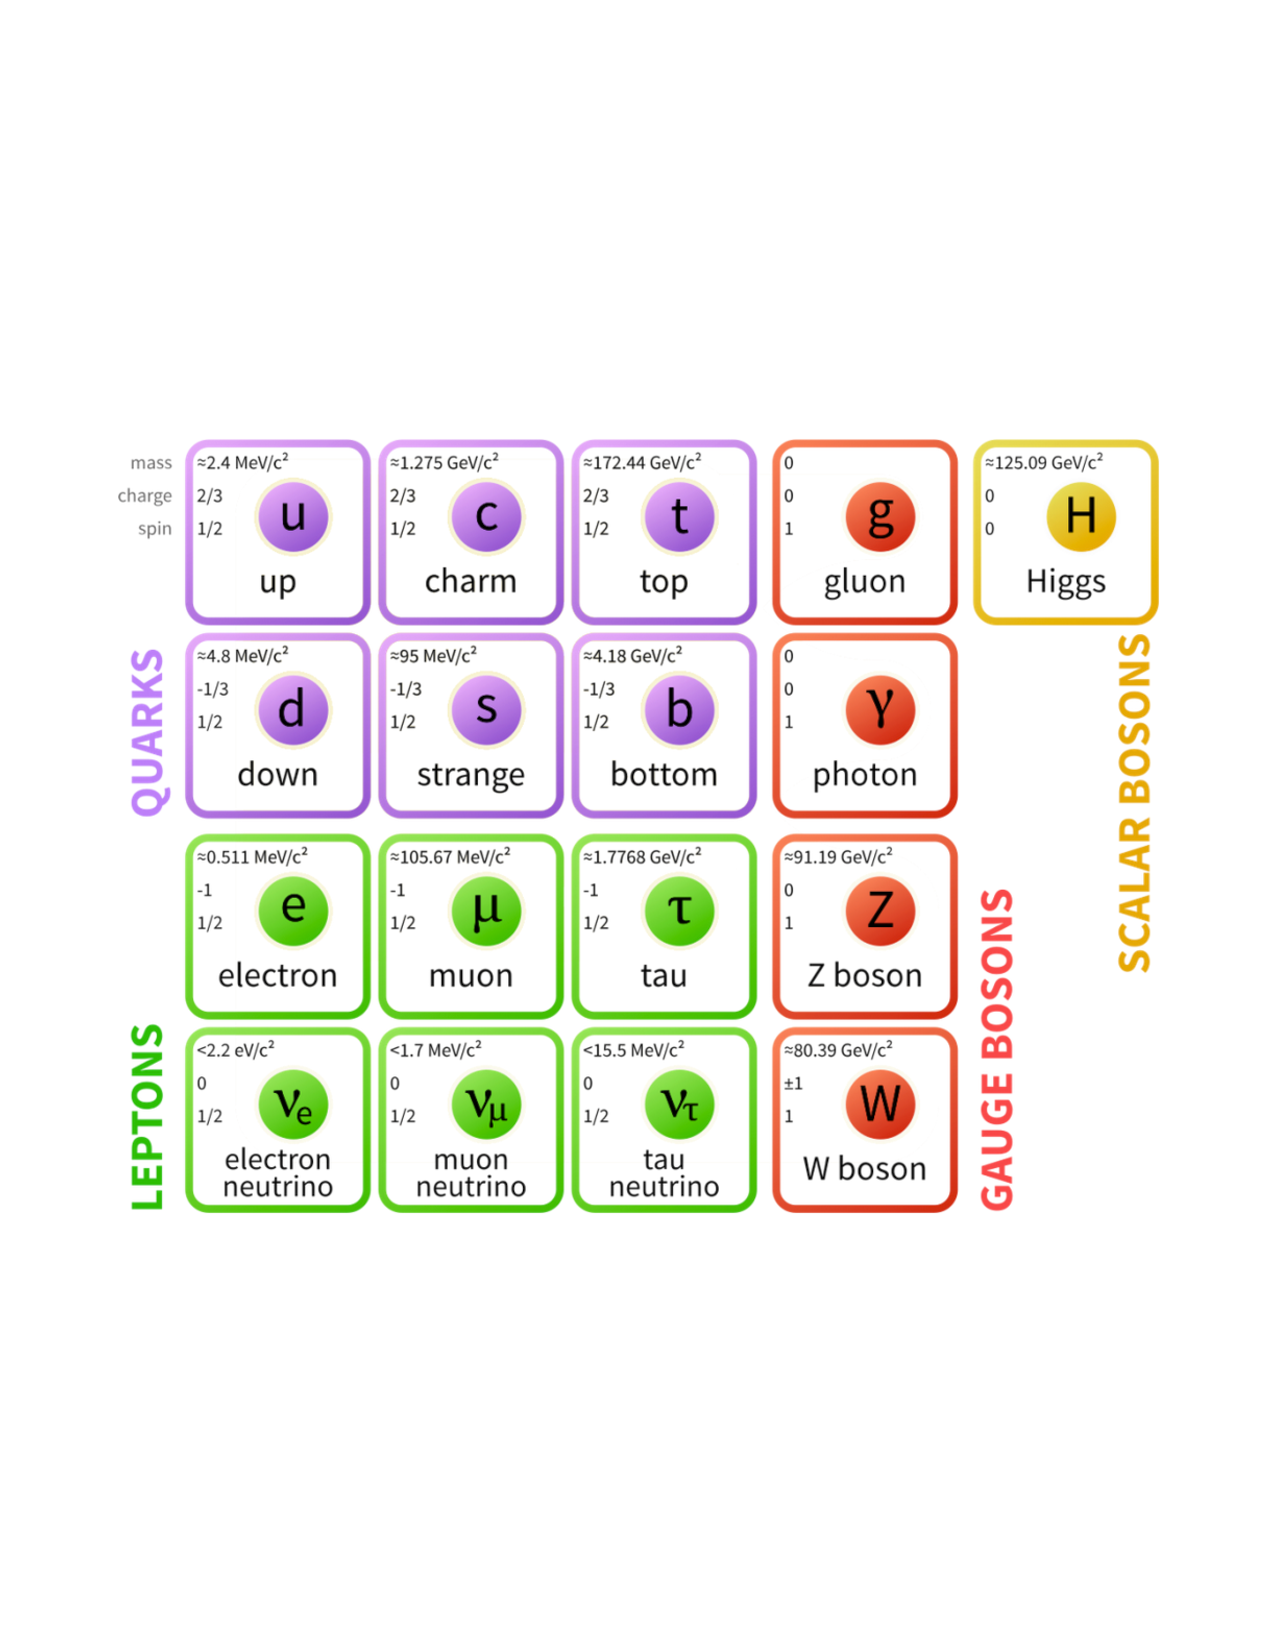
\includegraphics[width=1.0\textwidth]{smdiagram.pdf}
\caption{Fundamental particles of the Standard Model~\cite{modellinginvisible}.}
\label{fig:SM}
\end{figure}






\subsection{Quantum Chromodynamics}\label{secSM:ch1}
